\section{Difference of Networks}
\label{app:explaining_io_convex_nns}

In this appendix, we empirically investigate two questions using a simple image classification task:
\begin{enumerate}
    \item[(A)] Are the faithful saliency maps observed in \cref{sec:experiments} a general property of monotone neural networks?
    \item[(B)] Can we directly train a \emph{difference-of-two monotone neural networks}, rather than obtaining such a decomposition by splitting a general architecture? 
\end{enumerate}

We introduced the two resulting architectures as DMs and DICs as well as their inverted-input variations DMINs and DICINs in \cref{subsec:dc_network_training_methods}. \citetapp{AppSankaranarayanan2021CDINN} proposed an architecture similar to DICs as Convex Difference Neural Network (\emph{CDiNN}) in the context of optimal control.
Our experiments provide evidence that montone neural networks are inherently self-explanatory: ICNNs consistently focus on the most informative present and missing visual features in the image classification task. We remark that here we view ICNNs as monotone networks on an affine transformation of the input embodied by the first network layer. The gradients of the DICIN models clearly separate their concerns: The gradients of the $g$-model provide factual, while the gradients of the $h$-model provide counterfactual explanations.
Moreover, all proposed network architectures achieve excellent test accuracy on MNIST.

\subsection{Experimental Setup} \label{subsec:dic_experiment}

We evaluate two representative architectures -- as rank-2 Maxout networks consistently outperformed standard ReLU networks in the difference setting, we settled with the Maxout variants of two classical neural network architectures. We remark that this choice aligns with the fact that the split-streams in \cref{sec:method} effectively are rank-2 Maxout networks.

\paragraph{\texttt{cnn\_maxout}}
A convolutional neural network with Maxout activations.
It consists of four convolutional layers with 32, 64, 128, and 128 channels, each using $3\times3$ kernels with padding 1 and batch normalization after every layer.
After flattening the network applies three fully connected layers with dimensions $6272 \rightarrow 1024 \rightarrow 256 \rightarrow 10$, applying rank-2 Maxout activations after each hidden layer.
In total, it contains approximately 1.2M parameters, including the Maxout expansion.

\paragraph{\texttt{mlp\_maxout}}
A wide multilayer perceptron that also employs Maxout units.
It comprises four fully connected layers with dimensions $784 \rightarrow 800 \rightarrow 800 \rightarrow 800 \rightarrow 10$, using rank-2 Maxout activations after each hidden layer and batch normalization after the first three layers.
This network contains approximately 4.2M parameters, including the Maxout expansion.

\paragraph{Restricting the weights}

To enforce non-negativity we replace weight matrices $W$ with trainable parameters $\tilde{W}$ and apply a positivity transform $p$ such that the effective weights are $p(\tilde{W})$.
We explored several choices for $p$ (\eg \emph{softplus}, exponential, square) and found that $p=\text{ReLU}$ yielded the best test accuracy when all $\tilde{W}$ were initialized by sampling from a Gaussian distribution and taking the absolute value.
As a technical note, we also apply $p$ to the scaling and shifting parameters of all \emph{batch normalization} layers, as well as to all biases.

Because non-negative weights can cause exploding activations, we use a small initialization scale for all base model weights and apply a weight decay of $10^{-3}$ in all experiments.

\subsection{Results} \label{subsec:dic_results}

\begin{table}[h!]
\centering
\caption{Test accuracy across restriction modes (\%). Values show median with [min, max] range over 10 runs.}
\label{tab:cdinn_acc}
\begin{tabular}{lcccccccc}
\toprule
Model & IC & Mon & None & DIC & DM & Diff\_None & DICIN & DMIN \\
\midrule
\texttt{mlp\_maxout} & \makecell{98.36 \\ \scriptsize [98.07, 98.69]} & \makecell{98.30 \\ \scriptsize [97.64, 98.49]} & \makecell{98.39 \\ \scriptsize [98.07, 98.63]} & \makecell{98.56 \\ \scriptsize [98.33, 98.96]} & \makecell{98.55 \\ \scriptsize [98.23, 98.71]} & \makecell{98.47 \\ \scriptsize [98.19, 98.72]} & \makecell{98.58 \\ \scriptsize [98.41, 98.84]} & \makecell{98.54 \\ \scriptsize [98.36, 98.65]} \\
\texttt{cnn\_maxout} & \makecell{99.16 \\ \scriptsize [98.86, 99.27]} & \makecell{98.50 \\ \scriptsize [98.19, 98.79]} & \makecell{99.19 \\ \scriptsize [98.61, 99.44]} & \makecell{97.94 \\ \scriptsize [97.81, 98.04]} & \makecell{98.06 \\ \scriptsize [97.99, 98.19]} & \makecell{97.94 \\ \scriptsize [97.72, 98.45]} & \makecell{98.17 \\ \scriptsize [97.96, 98.34]} & \makecell{98.28 \\ \scriptsize [98.17, 98.54]} \\
\bottomrule
\end{tabular}
\end{table}

\Cref{tab:cdinn_acc} reports the median test accuracies of all considered architectures across 10 trainings with different random seeds. As a baseline we also trained and evaluated the difference of two unrestricted models, denoted by 
Diff\_None as well as an unrestricted model, denoted by None. The highest test performances are observed from \texttt{cnn\_maxout} None and IC models, reaching a median accuracy of $99.19\%$ and $99.16\%$ respectively. We remark that all our models achieve strong test accuracies.

For the \texttt{mlp\_maxout} the split variants DIC and DM outperform their respective single model counterparts IC and Mon. We assume that the strong inductive biases underlying a single \texttt{cnn\_maxout} model that are favorable for the MNIST task are a reason why this does not translate to the \texttt{cnn\_maxout} base model.
For both basemodels the inverted-input mode boosts the difference-of-two architecture.

In case of \texttt{mlp\_maxout} the IC and Mon are competitive with the unrestricted base model, while the test results are more seed-dependent for the restricted models and show higher variance. All the difference-of-two variants outperform the base model.

In case of \texttt{cnn\_maxout}, the IC variant achieves a surprisingly high median test accuracy of $99.16 \%$ comparable to the performance of the unrestricted baseline, even showing better minimal test accuracy than the baseline.
All the difference-of-two variants achieve strong, but unambiguously worse test accuracies compared to the single-model variants.

\begin{figure}[H]
    \centering
    \begin{subfigure}[b]{0.09\textwidth}
        \centering
        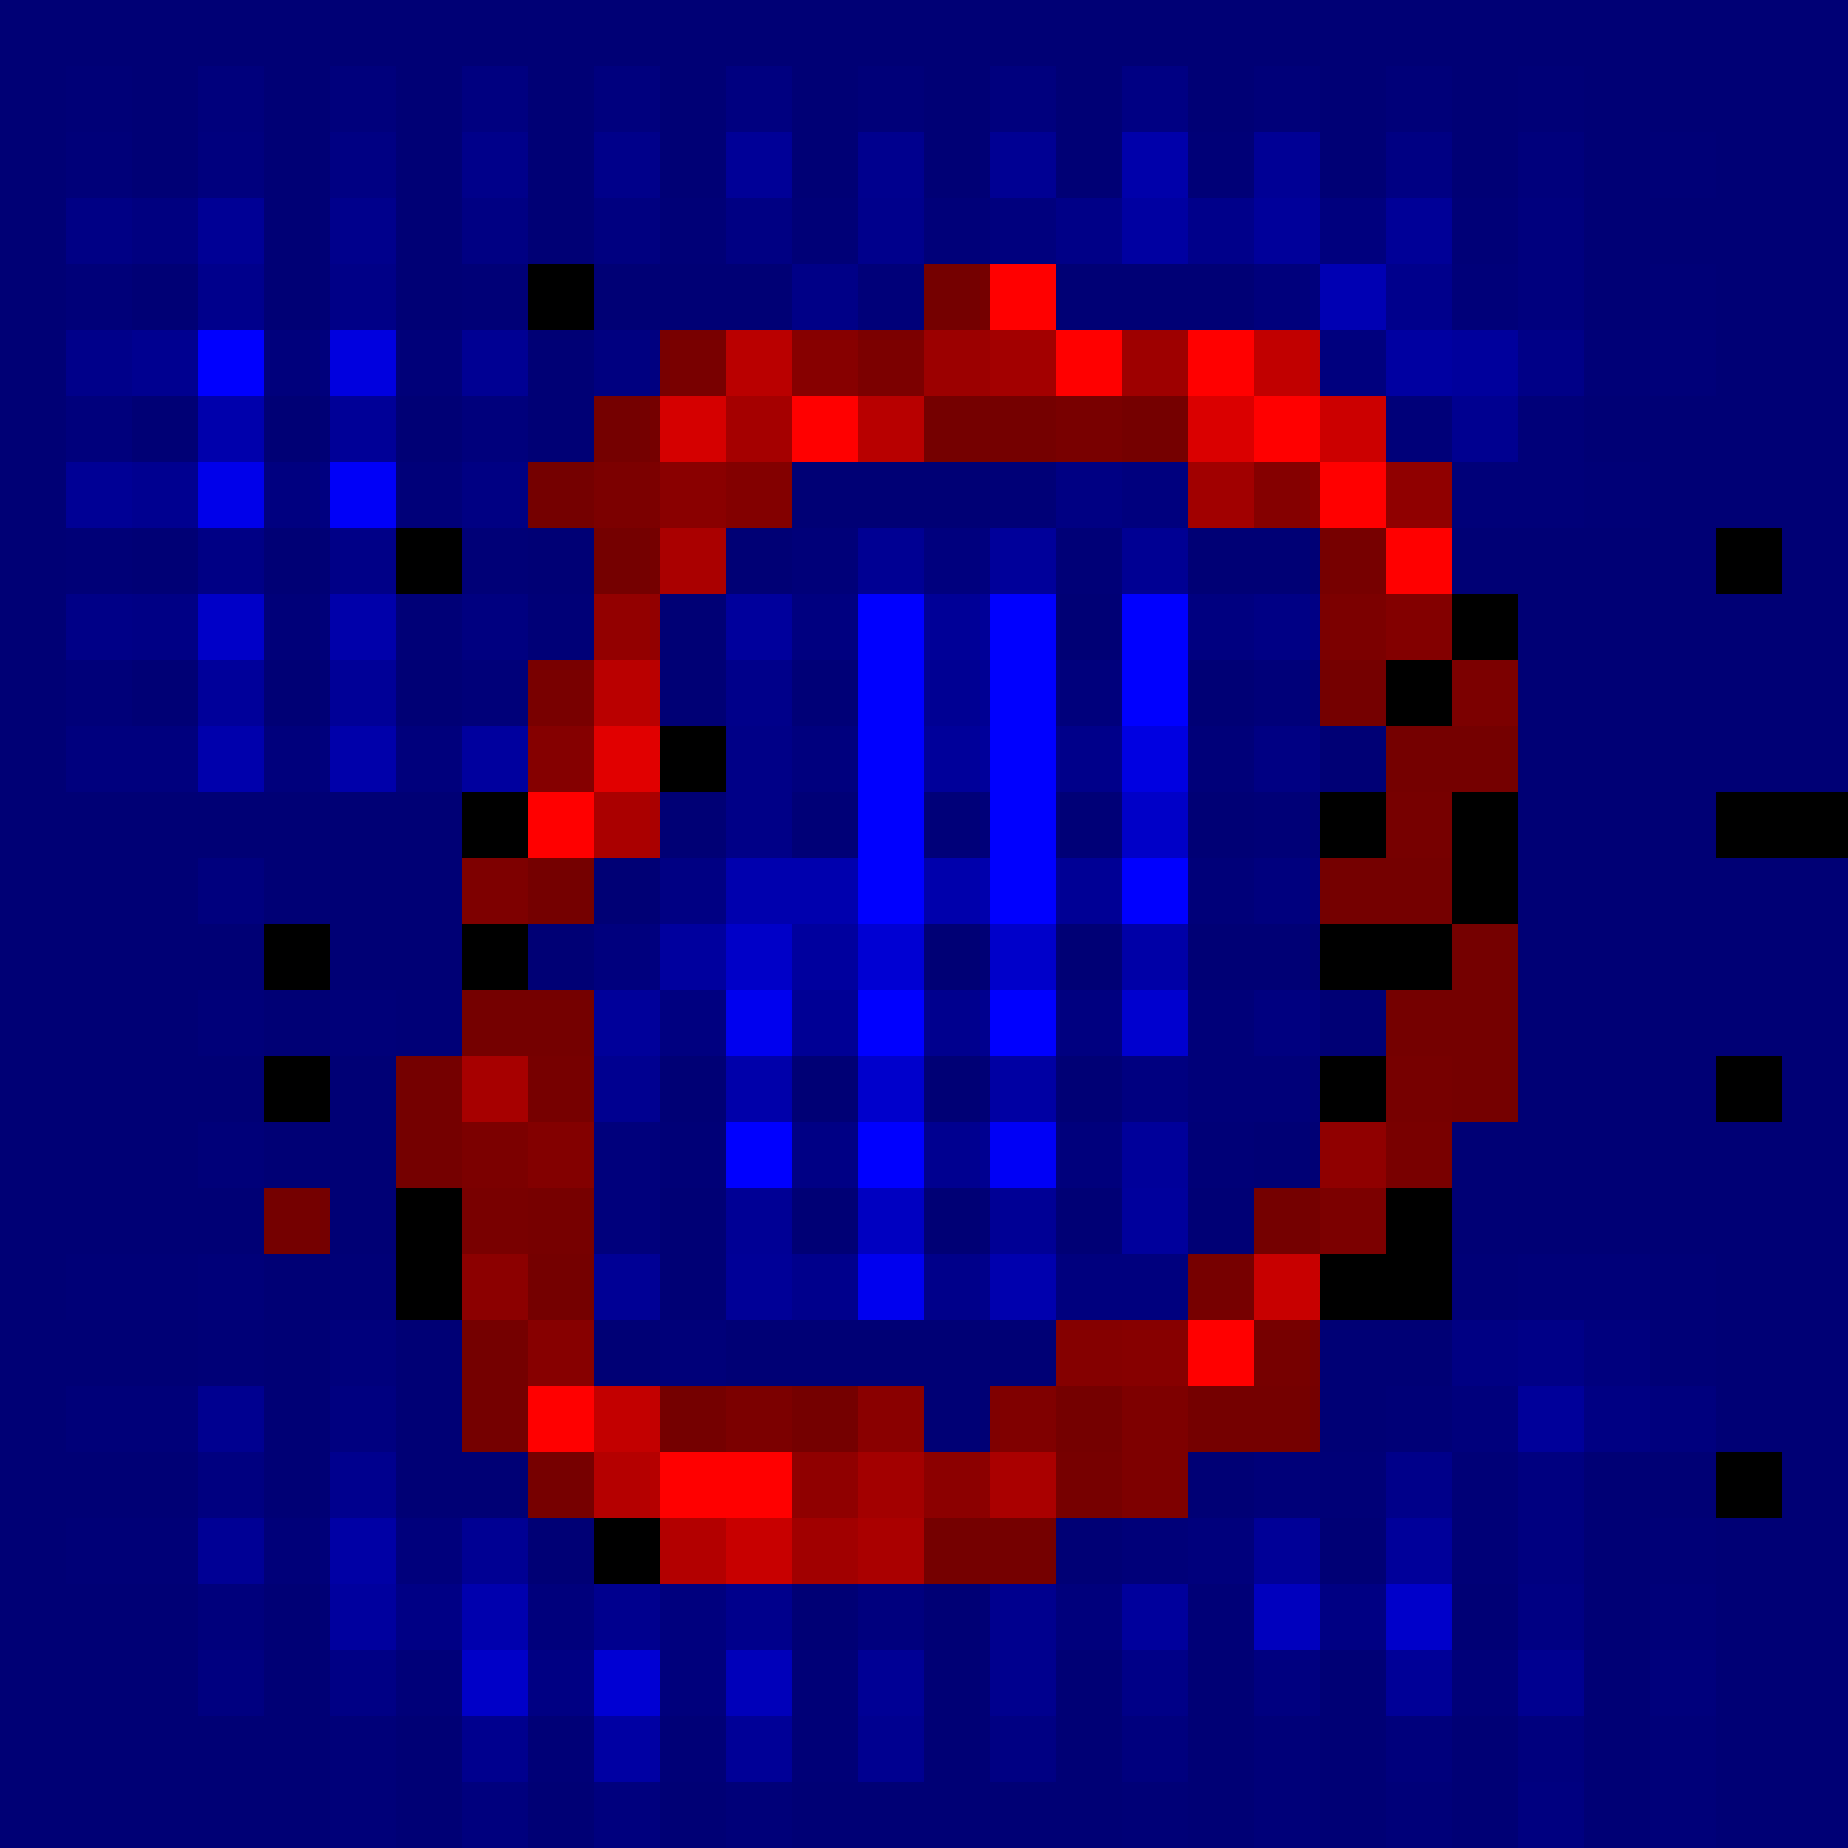
\includegraphics[width=\textwidth]{figures/mnist_ic_saliency/saliency_threshold_wrt_0_bright.png}
    \end{subfigure}
    \begin{subfigure}[b]{0.09\textwidth}
        \centering
        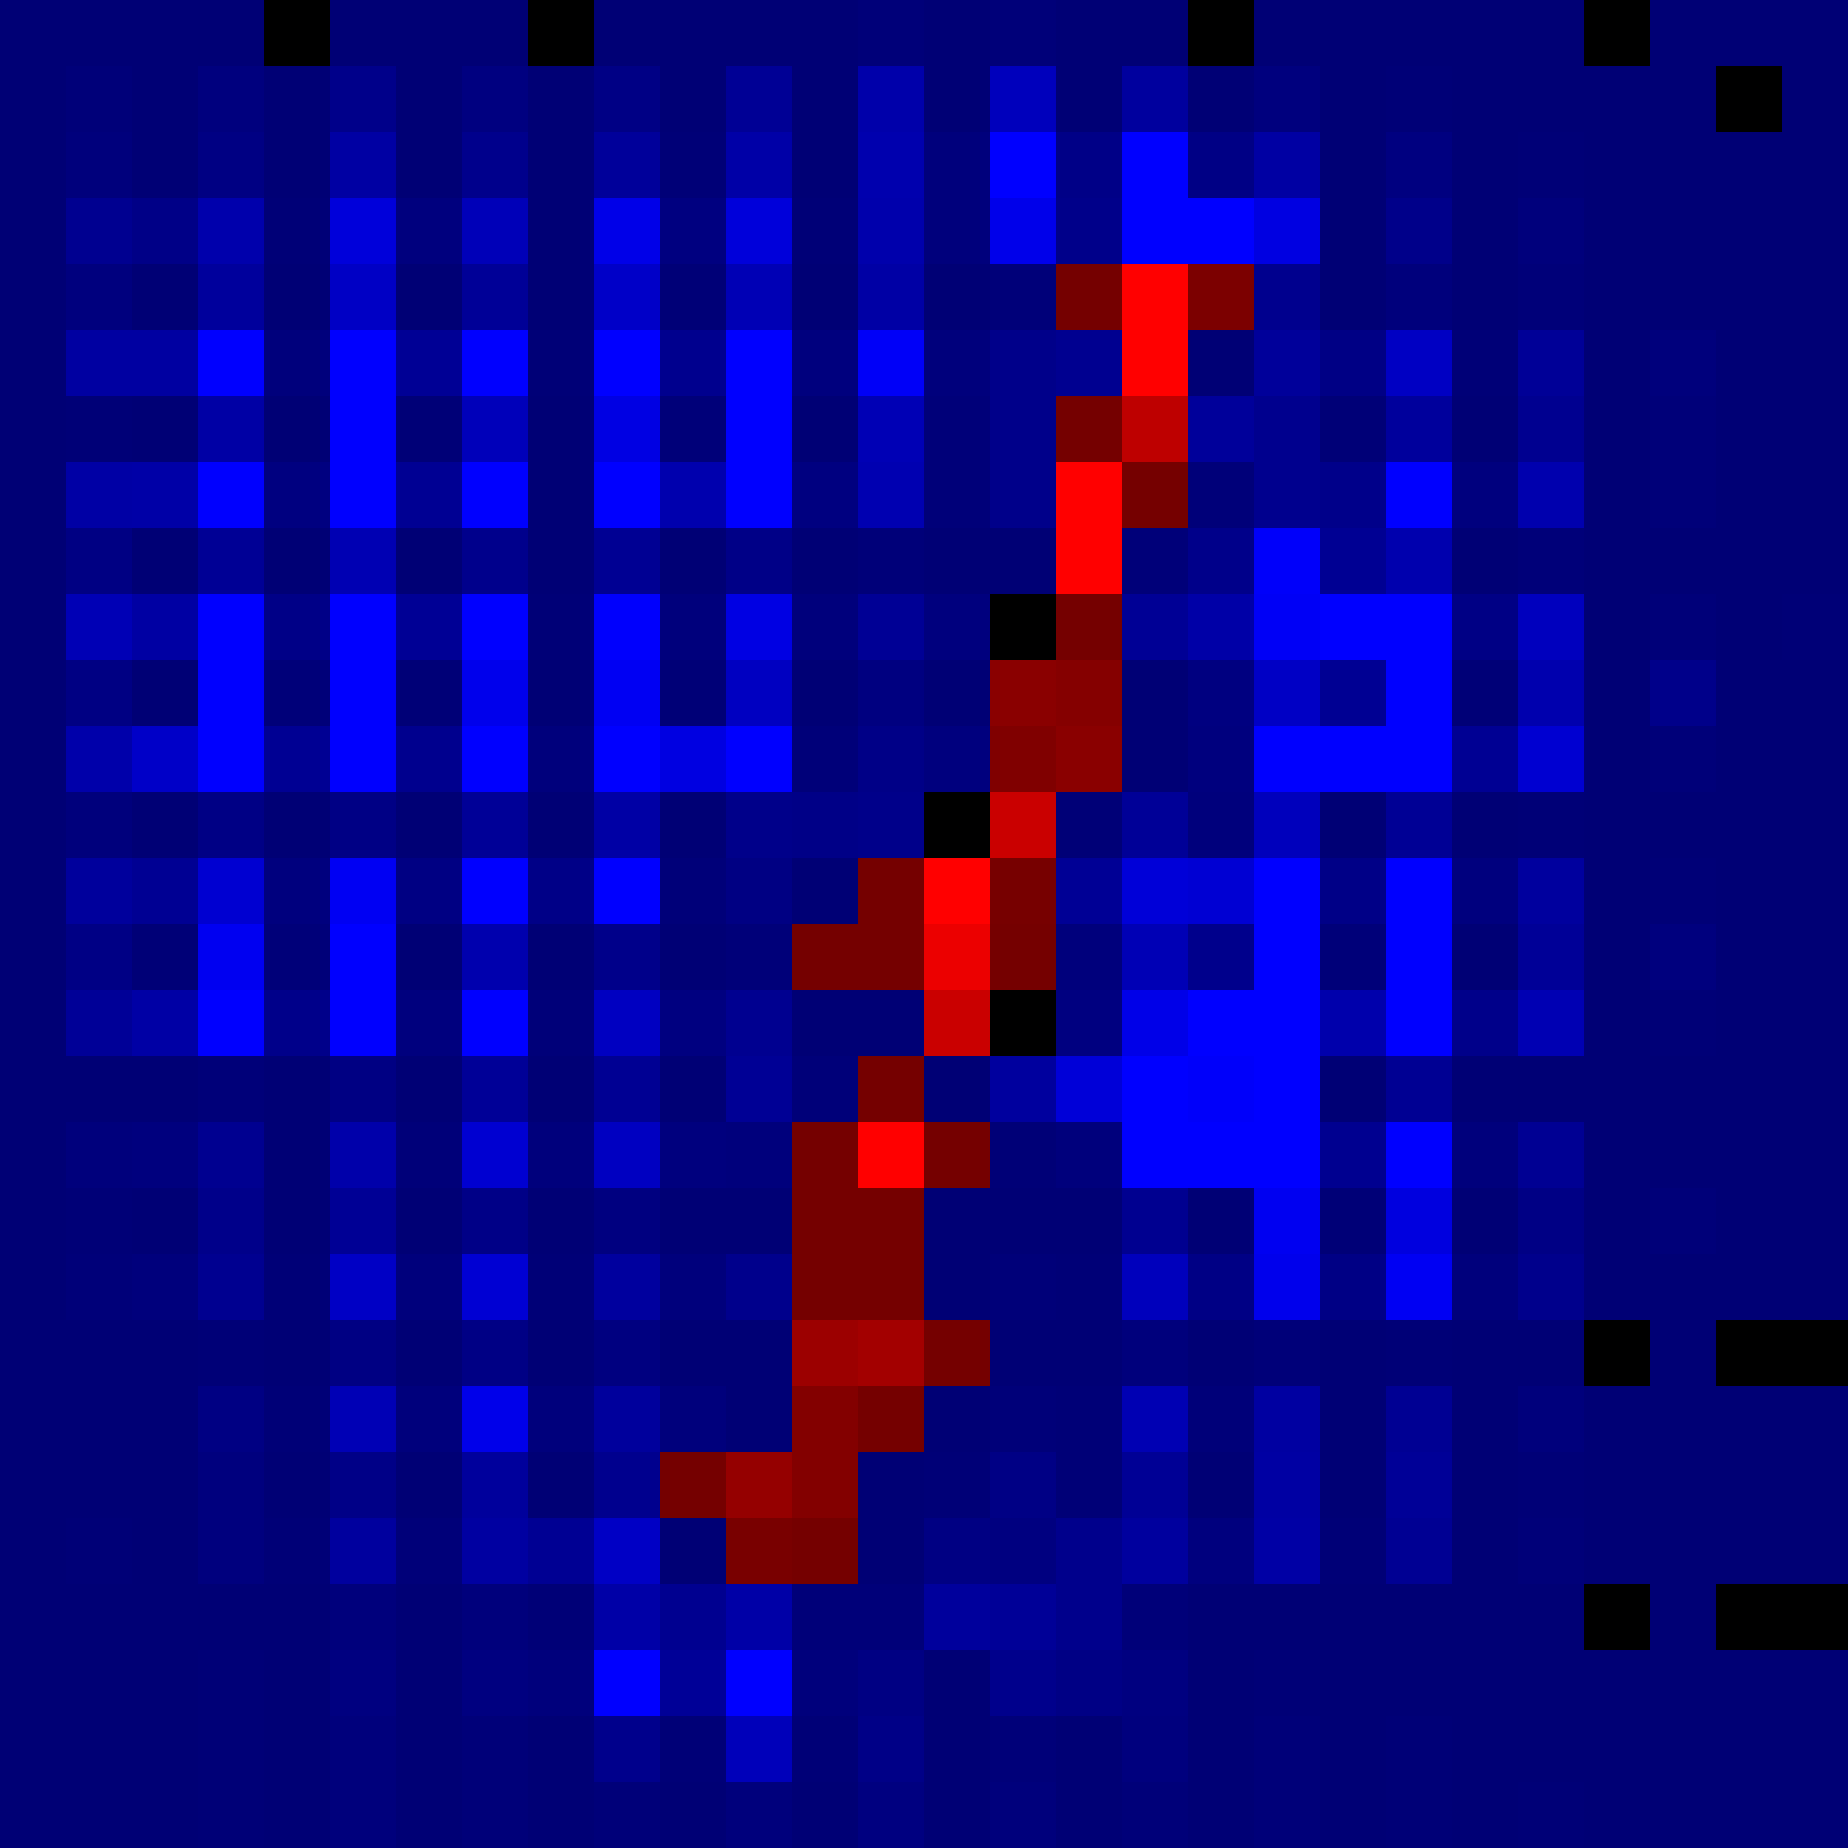
\includegraphics[width=\textwidth]{figures/mnist_ic_saliency/saliency_threshold_wrt_1_bright.png}
    \end{subfigure}
    \begin{subfigure}[b]{0.09\textwidth}
        \centering
        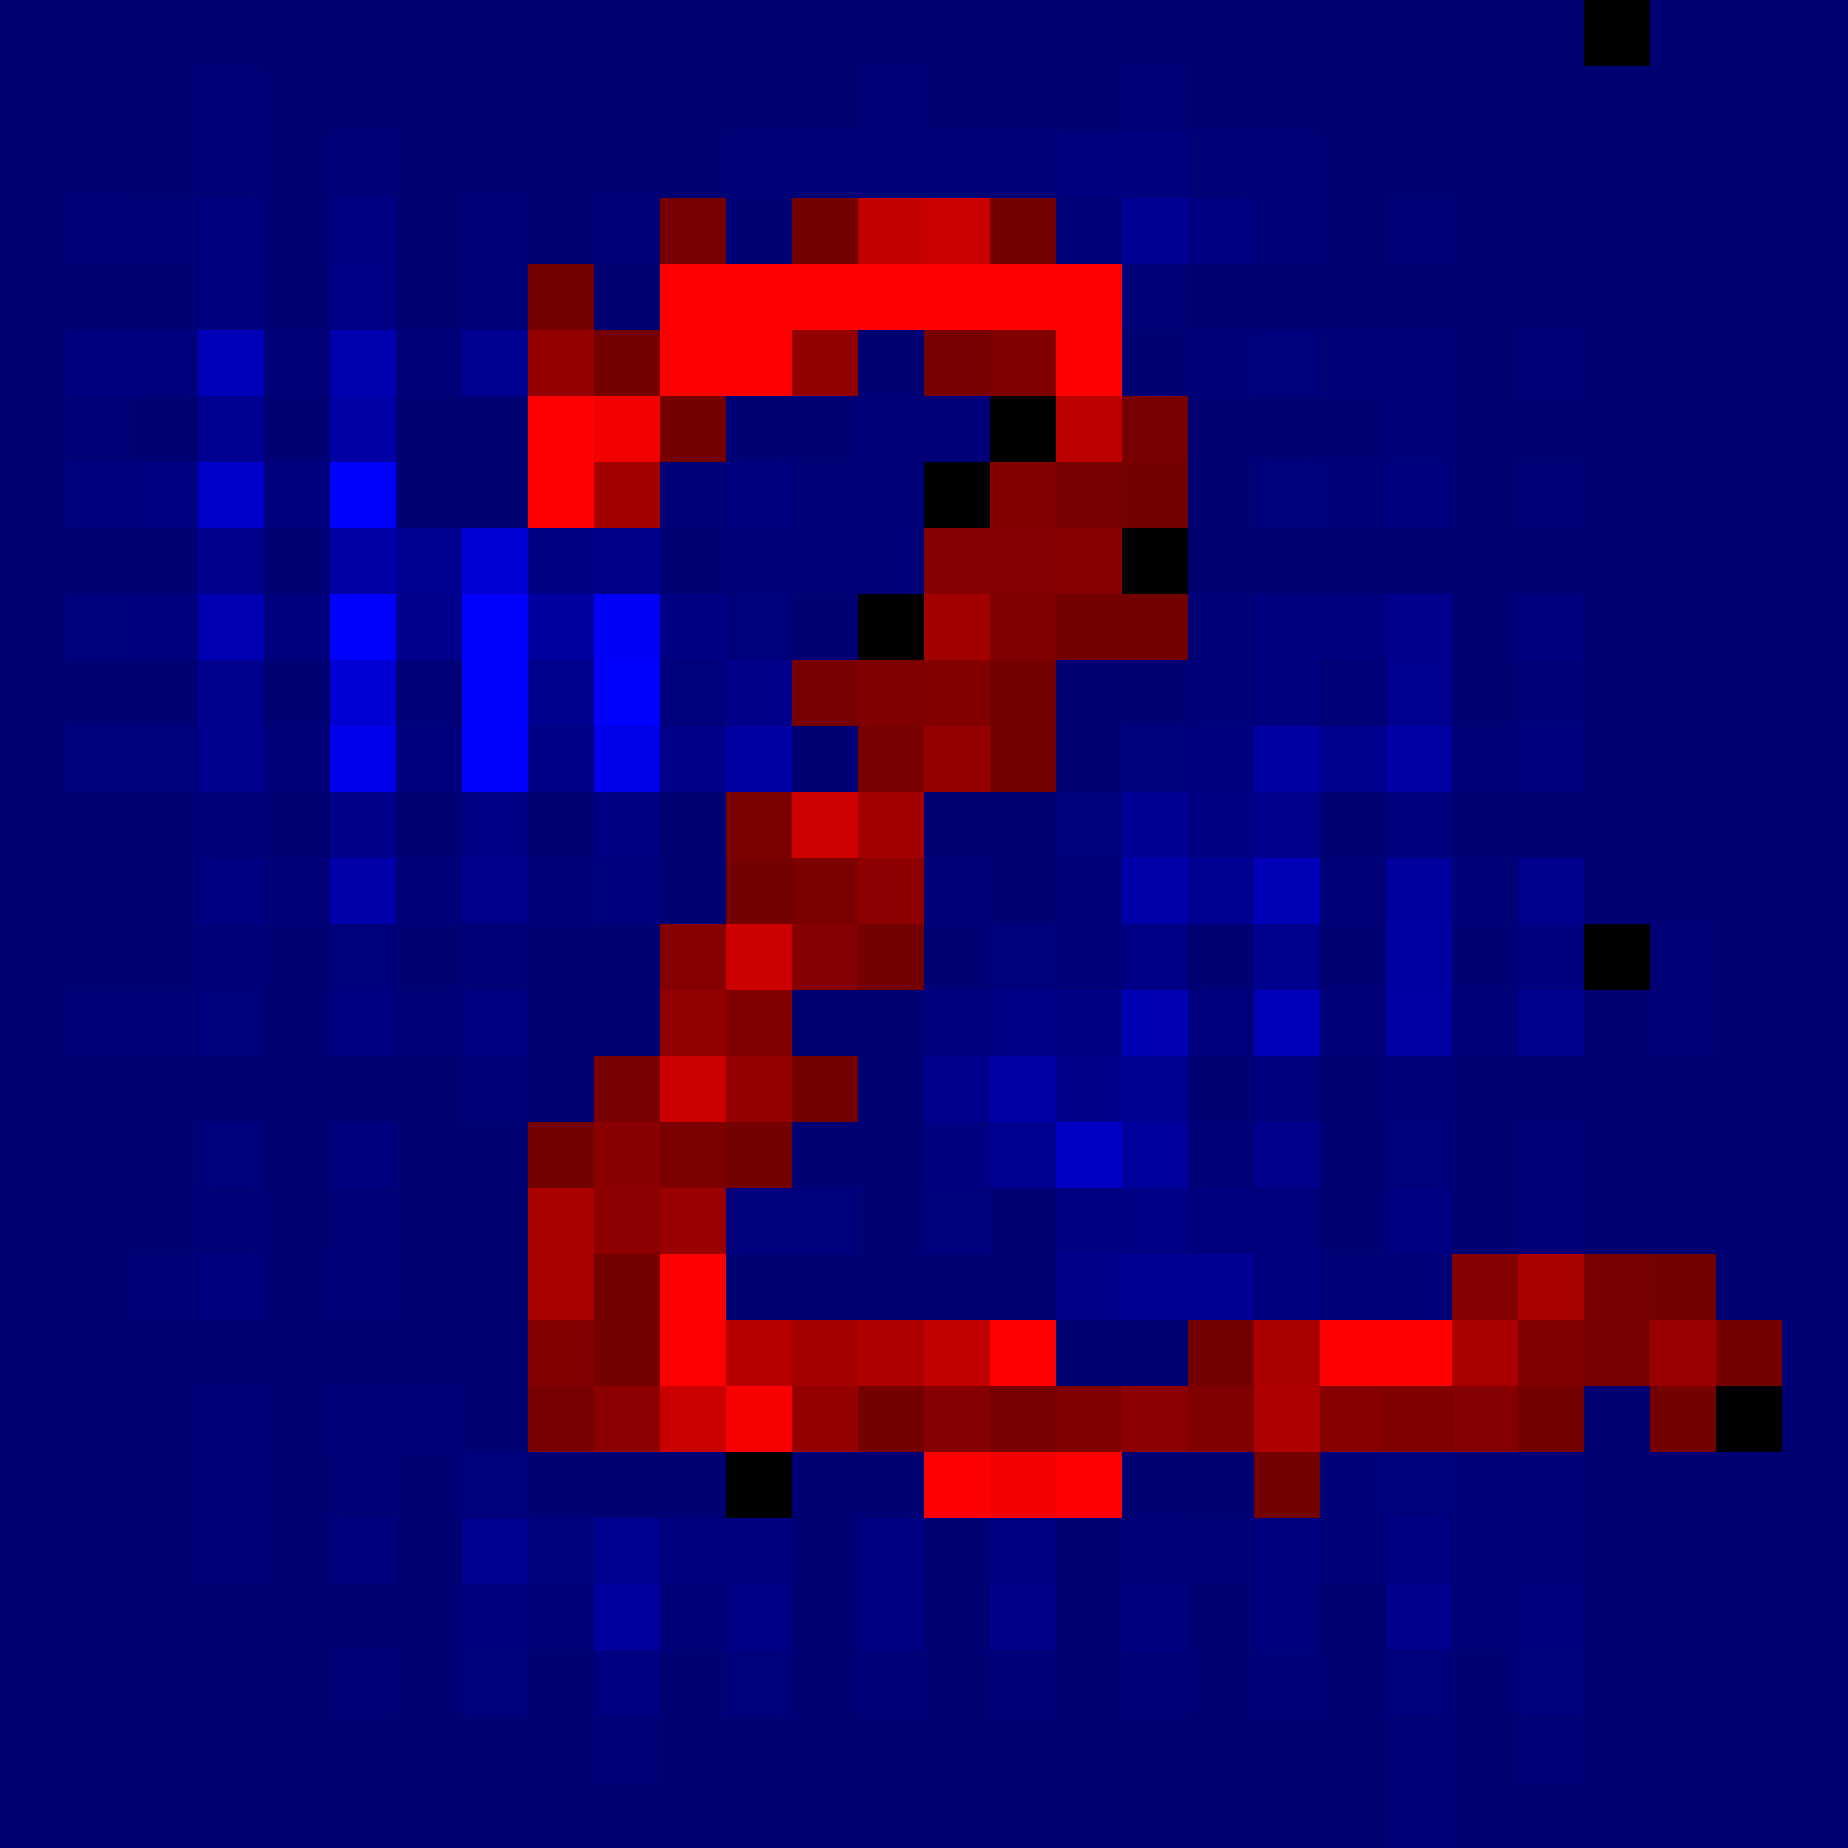
\includegraphics[width=\textwidth]{figures/mnist_ic_saliency/saliency_threshold_wrt_2_bright.png}
    \end{subfigure}
    \begin{subfigure}[b]{0.09\textwidth}
        \centering
        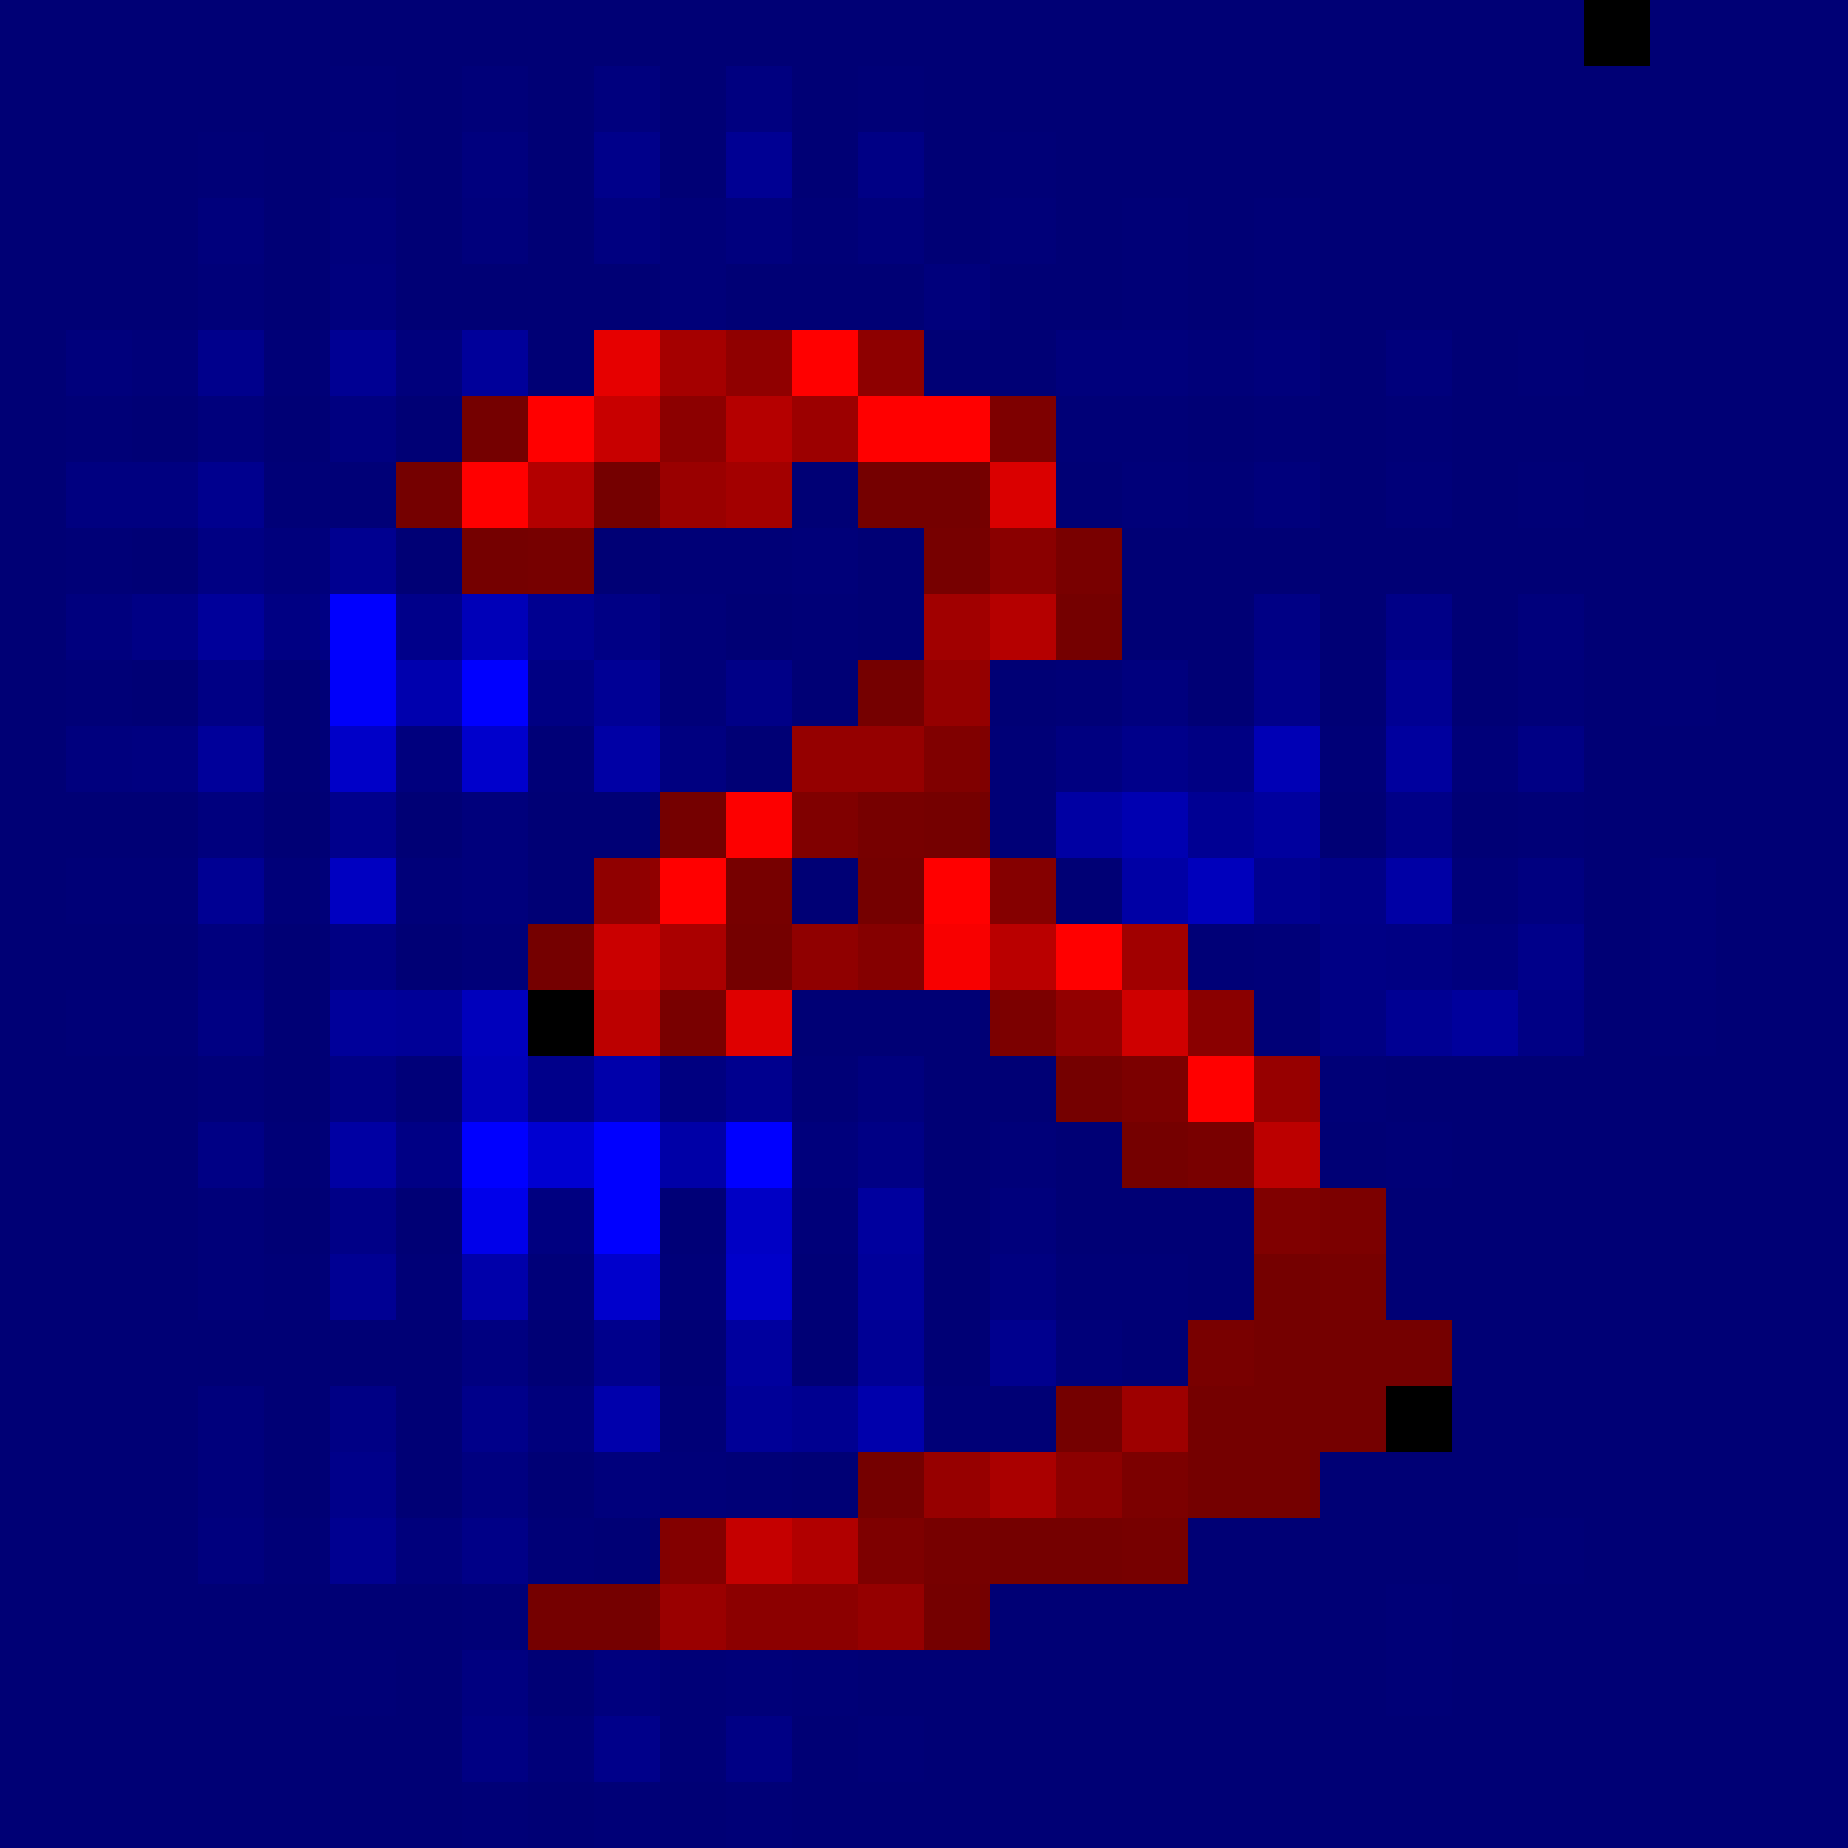
\includegraphics[width=\textwidth]{figures/mnist_ic_saliency/saliency_threshold_wrt_3_bright.png}
    \end{subfigure}
    \begin{subfigure}[b]{0.09\textwidth}
        \centering
        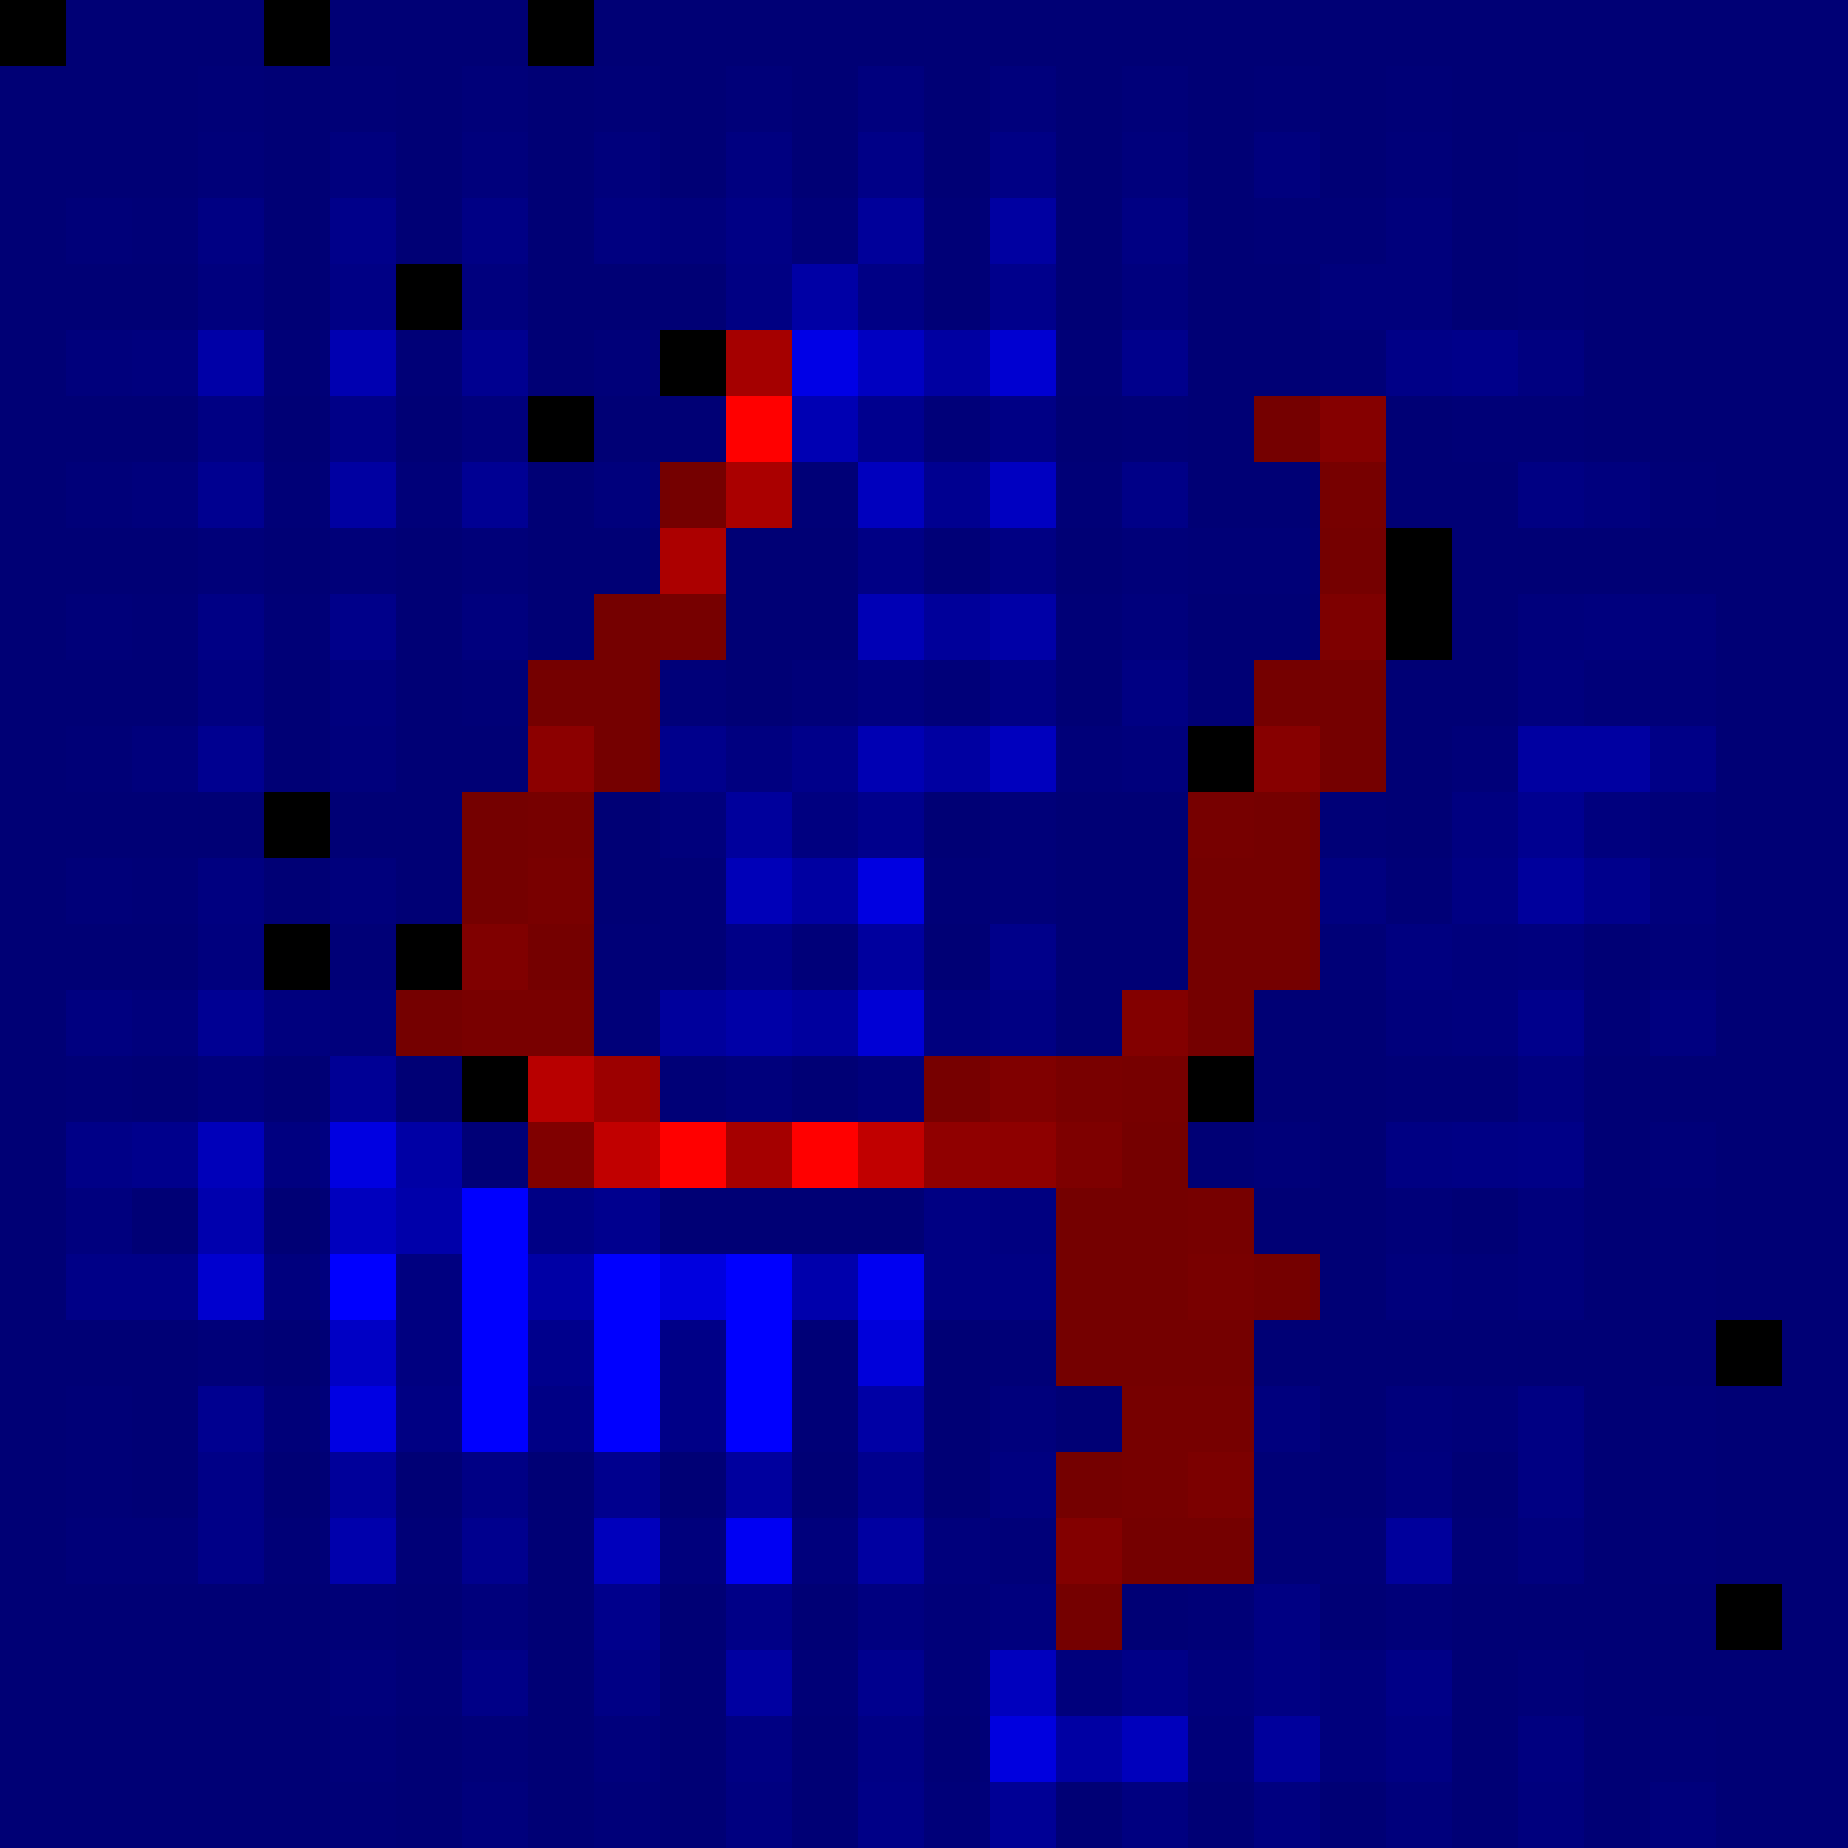
\includegraphics[width=\textwidth]{figures/mnist_ic_saliency/saliency_threshold_wrt_4_bright.png}
    \end{subfigure}
    \begin{subfigure}[b]{0.09\textwidth}
        \centering
        
\includegraphics[width=\textwidth]{figures/mnist_ic_saliency/saliency_threshold_wrt_5_bright.png}
    \end{subfigure}
    \begin{subfigure}[b]{0.09\textwidth}
        \centering
        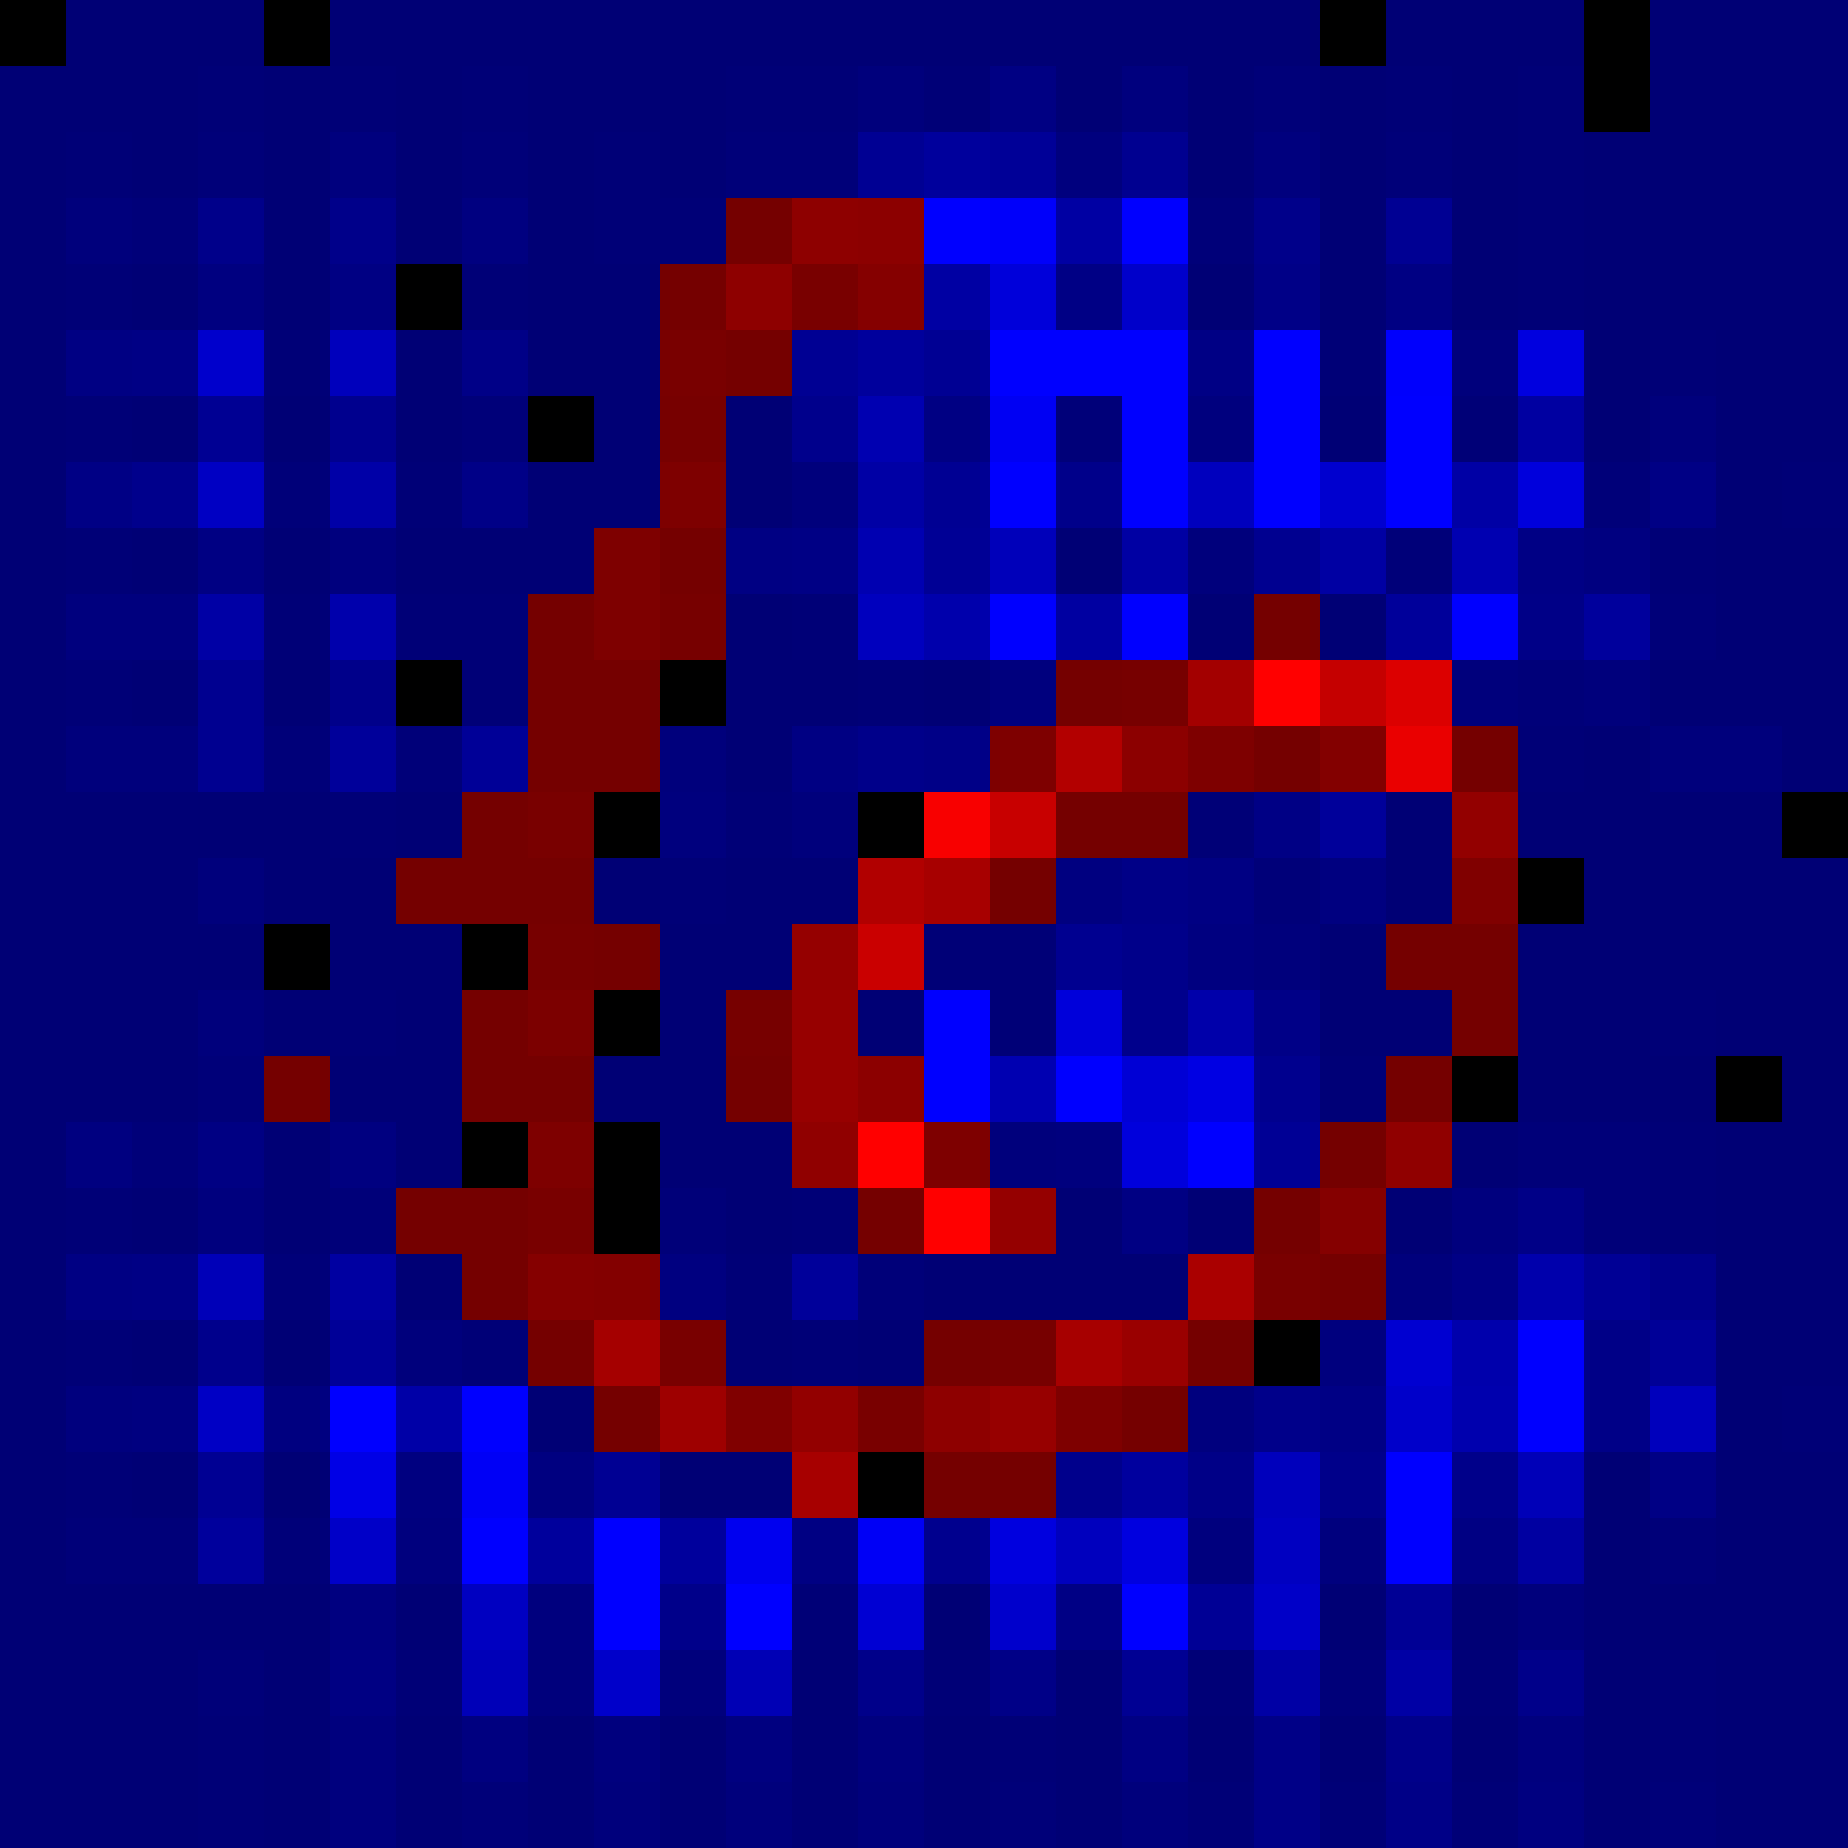
\includegraphics[width=\textwidth]{figures/mnist_ic_saliency/saliency_threshold_wrt_6_bright.png}
    \end{subfigure}
    \begin{subfigure}[b]{0.09\textwidth}
        \centering
        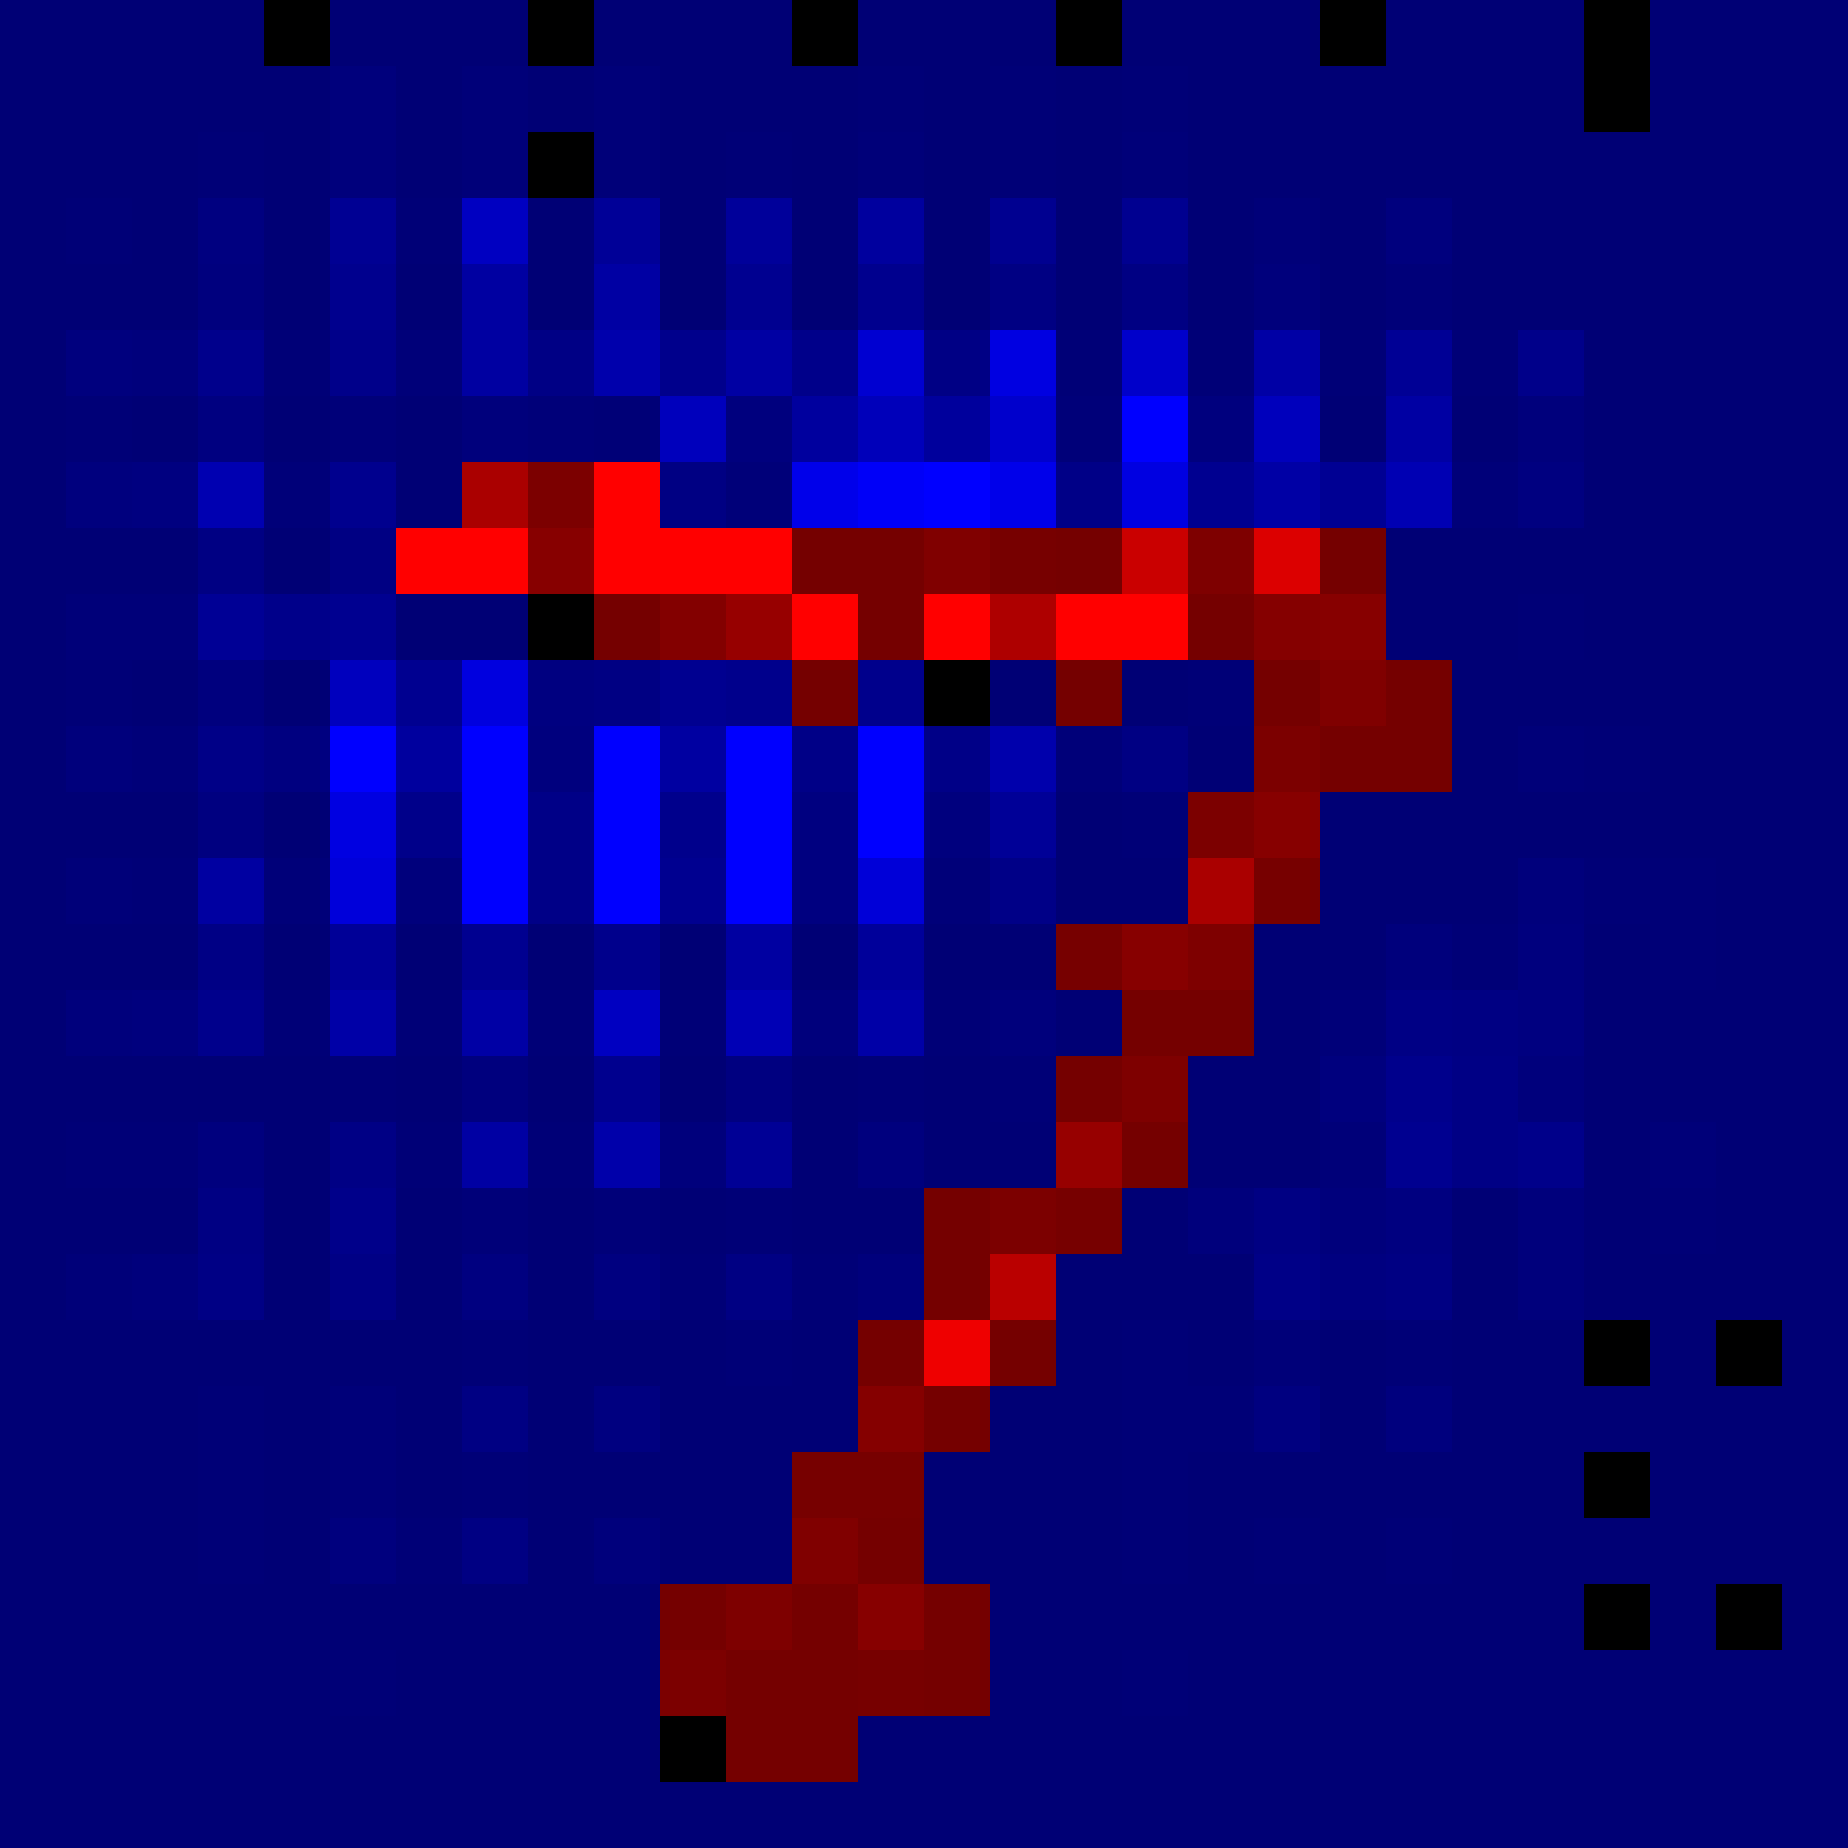
\includegraphics[width=\textwidth]{figures/mnist_ic_saliency/saliency_threshold_wrt_7_bright.png}
    \end{subfigure}
    \begin{subfigure}[b]{0.09\textwidth}
        \centering
        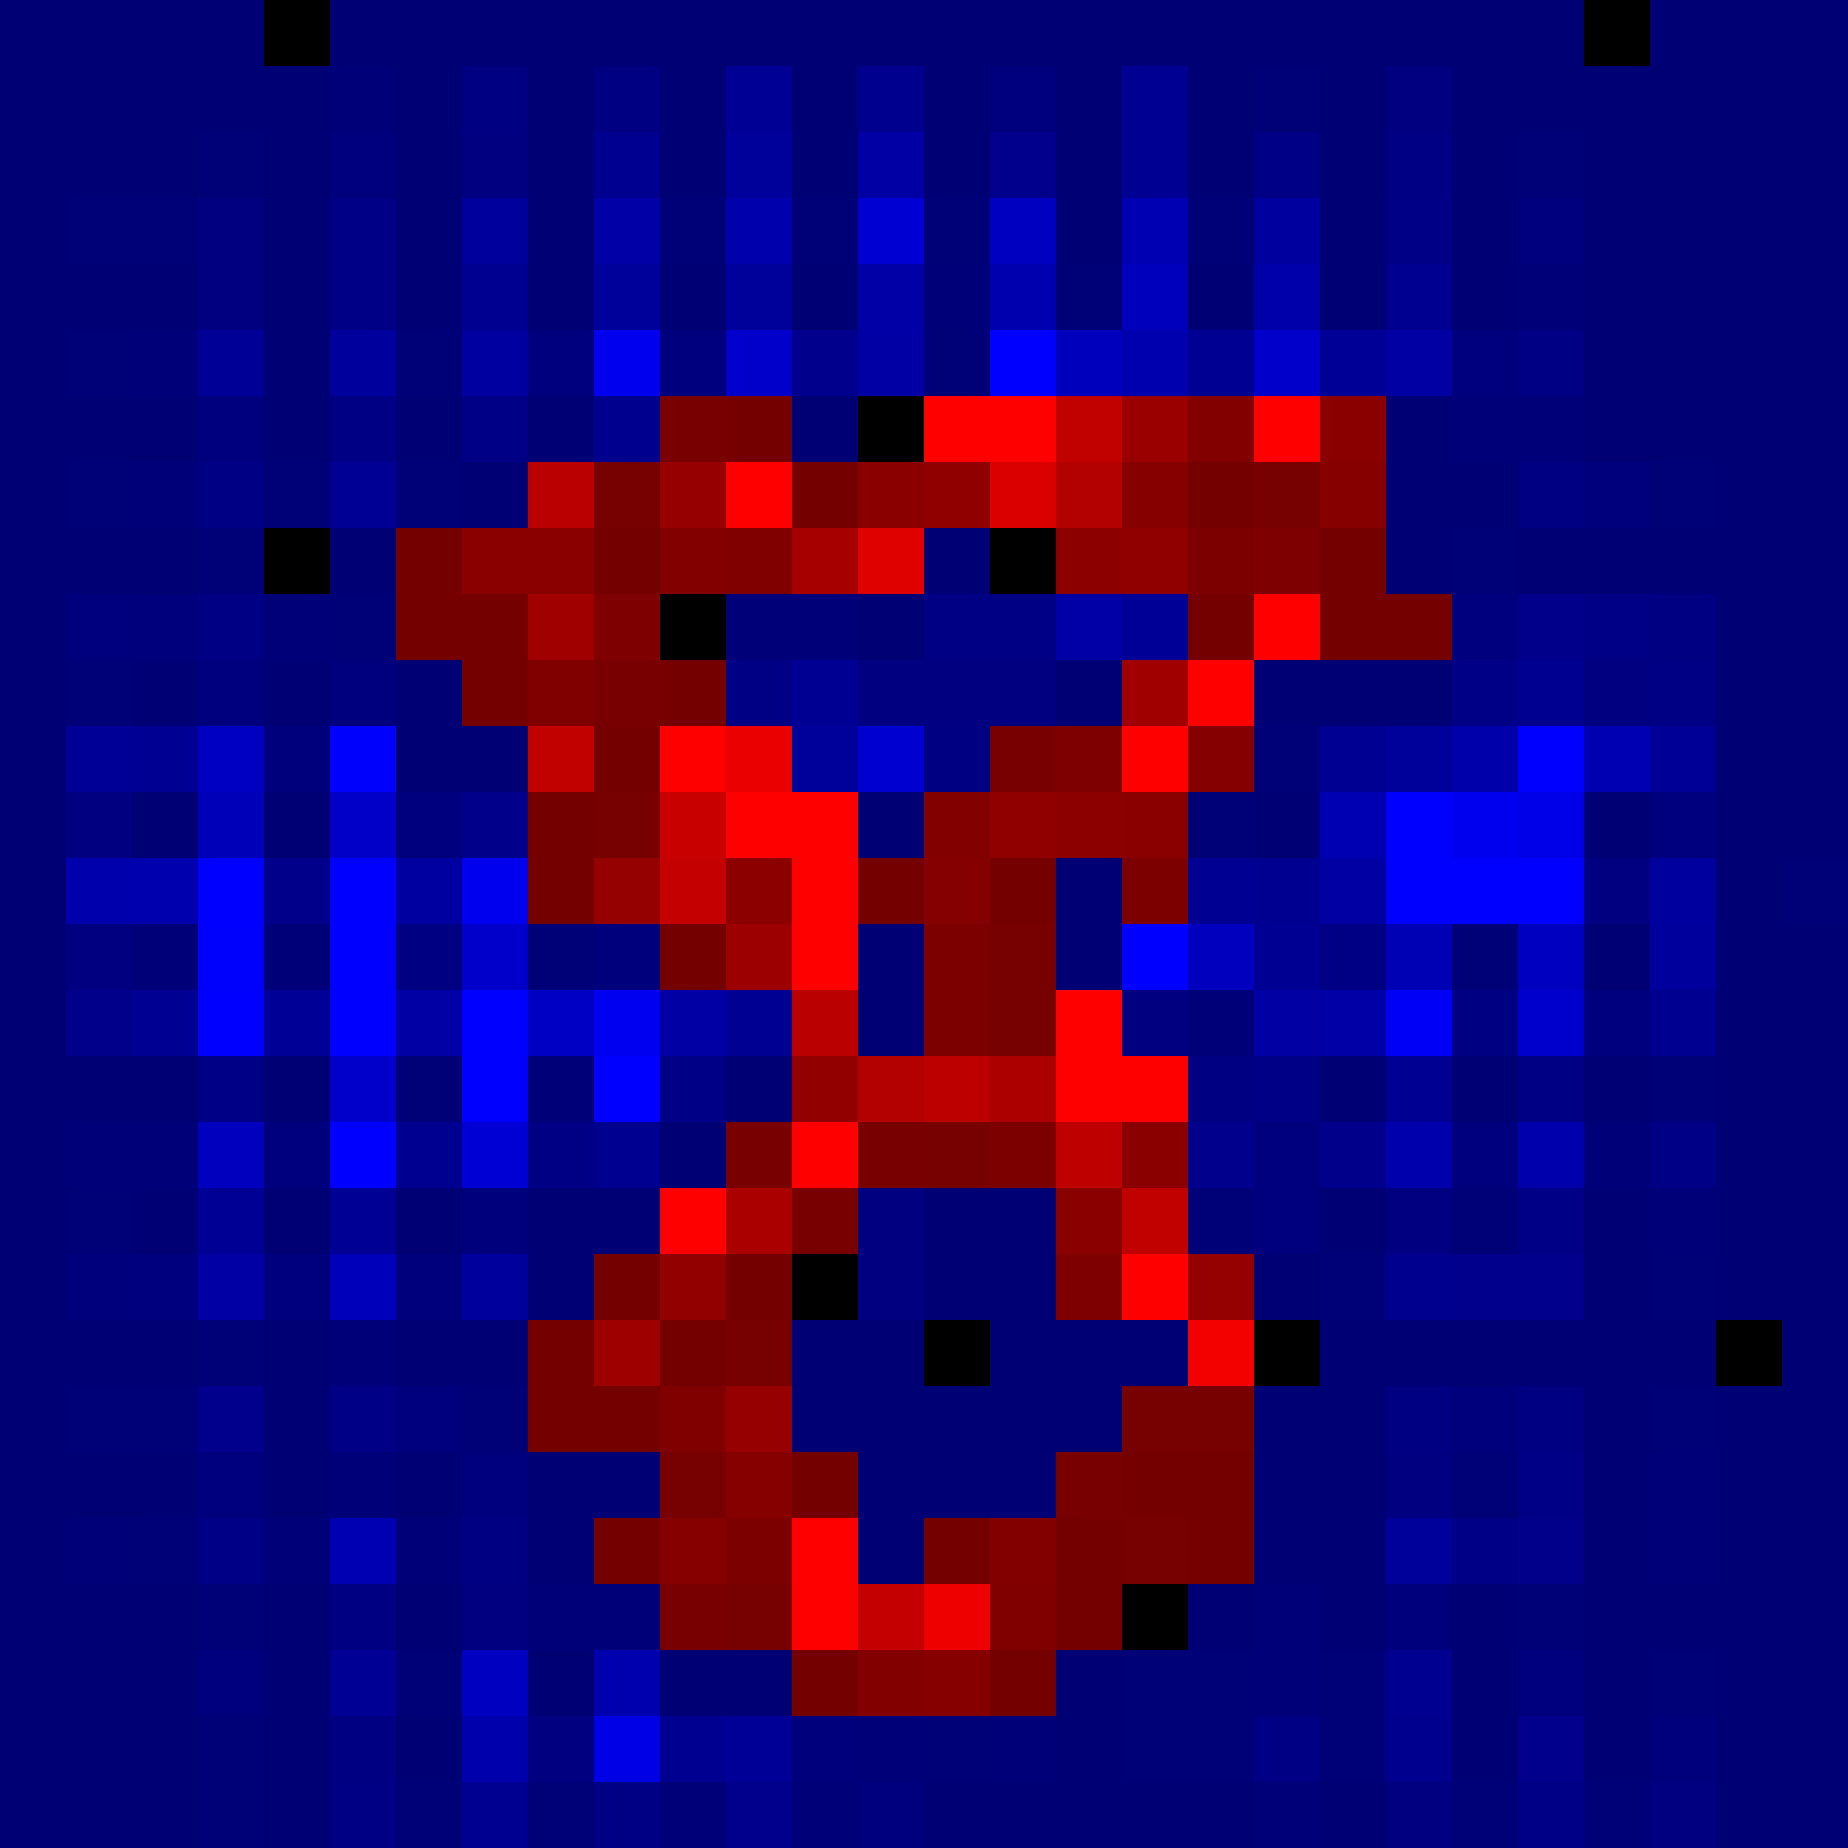
\includegraphics[width=\textwidth]{figures/mnist_ic_saliency/saliency_threshold_wrt_8_bright.png}
    \end{subfigure}
    \begin{subfigure}[b]{0.09\textwidth}
        \centering
        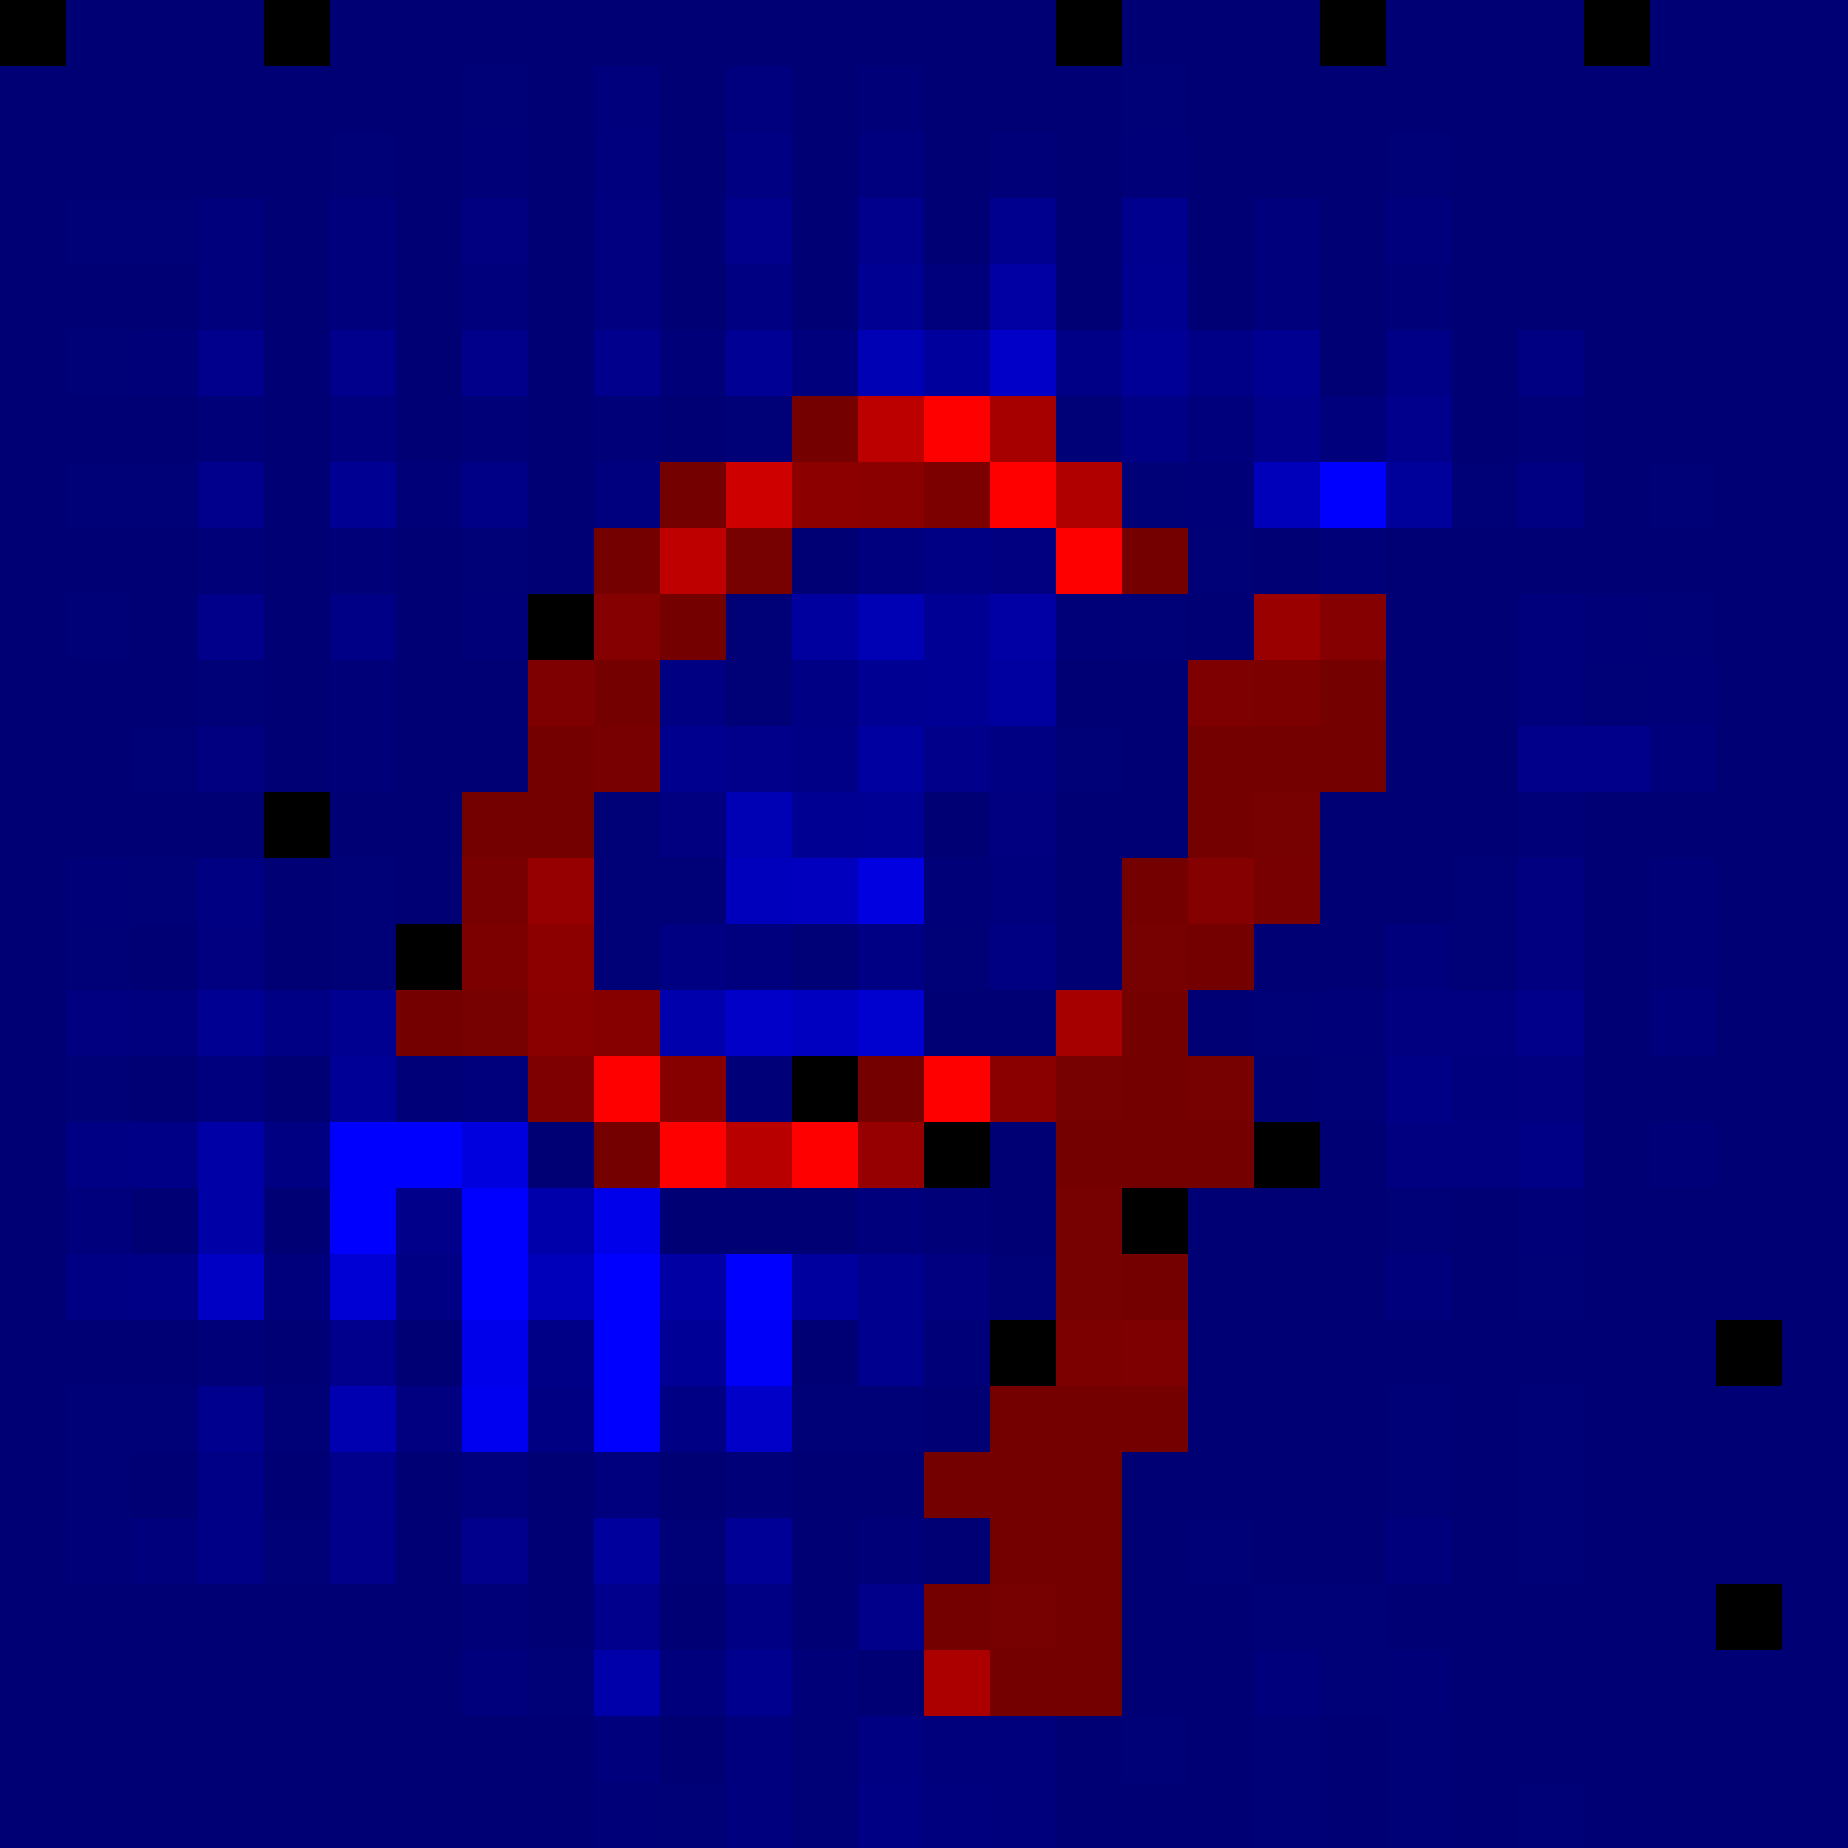
\includegraphics[width=\textwidth]{figures/mnist_ic_saliency/saliency_threshold_wrt_9_bright.png}
    \end{subfigure}

    \vspace{0.5cm}

    \begin{subfigure}[b]{0.09\textwidth}
        \centering
        
\includegraphics[width=\textwidth]{figures/mnist_ic_saliency/original_0.png}
        \caption*{\scriptsize Label 0}
    \end{subfigure}
    \begin{subfigure}[b]{0.09\textwidth}
        \centering
        
\includegraphics[width=\textwidth]{figures/mnist_ic_saliency/original_1.png}
        \caption*{\scriptsize Label 1}
    \end{subfigure}
    \begin{subfigure}[b]{0.09\textwidth}
        \centering
        
\includegraphics[width=\textwidth]{figures/mnist_ic_saliency/original_2.png}
        \caption*{\scriptsize Label 2}
    \end{subfigure}
    \begin{subfigure}[b]{0.09\textwidth}
        \centering
        
\includegraphics[width=\textwidth]{figures/mnist_ic_saliency/original_3.png}
        \caption*{\scriptsize Label 3}
    \end{subfigure}
    \begin{subfigure}[b]{0.09\textwidth}
        \centering
        
\includegraphics[width=\textwidth]{figures/mnist_ic_saliency/original_4.png}
        \caption*{\scriptsize Label 4}
    \end{subfigure}
    \begin{subfigure}[b]{0.09\textwidth}
        \centering
        
\includegraphics[width=\textwidth]{figures/mnist_ic_saliency/original_5.png}
        \caption*{\scriptsize Label 5}
    \end{subfigure}
    \begin{subfigure}[b]{0.09\textwidth}
        \centering
        
\includegraphics[width=\textwidth]{figures/mnist_ic_saliency/original_6.png}
        \caption*{\scriptsize Label 6}
    \end{subfigure}
    \begin{subfigure}[b]{0.09\textwidth}
        \centering
        
\includegraphics[width=\textwidth]{figures/mnist_ic_saliency/original_7.png}
        \caption*{\scriptsize Label 7}
    \end{subfigure}
    \begin{subfigure}[b]{0.09\textwidth}
        \centering
        
\includegraphics[width=\textwidth]{figures/mnist_ic_saliency/original_8.png}
        \caption*{\scriptsize Label 8}
    \end{subfigure}
    \begin{subfigure}[b]{0.09\textwidth}
        \centering
        
\includegraphics[width=\textwidth]{figures/mnist_ic_saliency/original_9.png}
        \caption*{\scriptsize Label 9}
    \end{subfigure}
    \caption{Input gradient visualizations of the \texttt{cnn\_maxout} IC model of ten digits with respect to their ground truth label. Top row: saliency maps. Bottom row: original images for each label. We colored positive and negative split-stream gradient values above threshold 0.2 red and blue respectively, where we colorized the ranking of the absolute values with an exponential decay.}

    \label{fig:mnist_ic_saliency}
\end{figure}


\cref{fig:mnist_ic_saliency} visualizes input gradients of the \texttt{cnn\_maxout} DIC model on representative test samples.
The gradients are mostly positive on the strokes and negative on the background, indicating that adding white pixels in certain regions and deleting stroke pixels would decrease the predicted confidence.
We observe that the hole of the ``0'', the gaps between the arches of ``3'' (distinguishing it from ``8'' and ``9''), the area between the belly of ``6'' and the arch of ``8'', and the vertical line and lower curve of ``7'' and ``8'' respectively, are all critical for classification.
It is remarkable that the positive gradient aligns precisely with the digit’s strokes.

However, the gradients of the \texttt{cnn\_maxout} IC do not exhibit class-dependent directional variation, in contrast to those of the \texttt{cnn\_maxout} DIC model.
\Cref{fig:mnist_split_ic_saliency_main} shows overlays of $g$- and $h$-network gradients (red and blue, respectively) for all classes on two test samples with correctly predicted ground-truth label ``3''.
Since the $h$-model receives $1 - x$ as input, a high gradient value (bright blue pixel) indicates that adding a white pixel at that location would increase the corresponding class logit.

Class ``1'' shows no $g$-gradient activity above the threshold, while the $g$-gradient for the ground-truth class ``3'' is strongest and follows the digit strokes most accurately.
For classes ``6'', ``8'', and ``9'', the $h$-gradients are dense between the arches of the ``3'', indicating that those missing pixels are discriminative for these classes.
In several cases, red gradients also align with the strokes of competing classes within the original digit structure.

\subsection{Conclusion}

Considering our results with small models on MNIST, we can answer both questions raised at the beginning of this appendix affirmatively.
Concerning question (B), we observed strong performance of our proposed DM and DIC models, in case of the small MLP even outperforming all single-model variants.
Concerning question (A), we even report better interpretability of the monotone and input-convex models in their single-model and difference-of-two setups compared to the DC decompositions of pretrained network architectures.
Indeed, we were not able to rigorously prove the disentanglement of concerns to factual and counterfactual features in the split-pairs of the pretrained VGG16 and ResNet18 models.
It is future work to translate our ideas from the proof of concept presented in this appendix to larger network architectures.